% !TeX root = ../courtade-kumar.tex
\usetikzlibrary{patterns}
\definecolor{progressrate}{RGB}{32,150,125}
\definecolor{progressfull}{HTML}{E27052}
\begin{figure}[H]
\centering
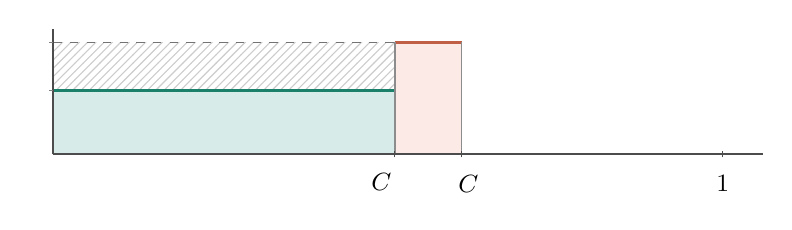
\begin{tikzpicture}[x=8.5cm,y=1.45cm,
    tick label/.style={font=\small}]
  \def\hbar{0.51}
  \def\htot{0.609840}
  \def\axisend{1.06}
  \def\srate{0.56}
  \def\qrate{0.98}
  \coordinate (HbarRate) at (\hbar,\srate);
  \coordinate (HbarFull) at (\hbar,\qrate);
  \coordinate (Htot) at (\htot,0);

  % Entropy is on the horizontal axis and the rate on the vertical axis.
  \fill[progressfull,opacity=0.15]
    (\hbar,0) rectangle (\htot,\qrate);
  \fill[progressrate,opacity=0.18]
    (0,0) rectangle (\hbar,\srate);
  \fill[pattern=north east lines,pattern color=black!20]
    (0,\srate) rectangle (\hbar,\qrate);

  \draw[dashed,black!55,line width=0.6pt]
    (0,\qrate) -- (\hbar,\qrate);
  \draw[progressrate!85!black,line width=1pt]
    (0,\srate) -- (\hbar,\srate);
  \draw[progressfull!85!black,line width=1pt]
    (\hbar,\qrate) -- (\htot,\qrate);
  \draw[black!45,line width=0.6pt]
    (\hbar,0) -- (\hbar,\qrate);
  \draw[black!45,line width=0.6pt]
    (\htot,0) -- (\htot,\qrate);

  \draw[black!70,line width=0.75pt] (0,0) -- (\axisend,0);
  \draw[black!70,line width=0.75pt] (0,0) -- (0,\qrate+0.12);
  \draw[black!50,line width=0.45pt] (-0.006,\srate) -- (0,\srate);
  \draw[black!50,line width=0.45pt] (-0.006,\qrate) -- (0,\qrate);
  \draw[black!70,line width=0.55pt] (\hbar,-0.028) -- (\hbar,0.028);
  \draw[black!70,line width=0.55pt] (\htot,-0.028) -- (\htot,0.028);
  \draw[black!70,line width=0.55pt] (1,-0.028) -- (1,0.028);

  \node[tick label,anchor=east,text=progressrate!90!black]
    at (-0.010,\srate) {$\sI$};
  \node[tick label,anchor=east,text=progressfull!90!black]
    at (-0.010,\qrate) {$\qI$};

  \node[tick label,anchor=north] at (0.49,-0.08) {$\tsent{C}$};
  \node[tick label,anchor=north] at (0.62,-0.10) {$\ent{C}$};
  \node[tick label,anchor=north] at (1,-0.10) {$1$};
\end{tikzpicture}
\captionsetup{font=small,name=Figure,labelformat=default,labelsep=period,labelfont=bf}
\caption{The hatched strip is the amount
  $(\qI-\sI)\tsent{C}$ subtracted from the strong data processing inequality $\qI\ent{C}$.}
\label{fig:progressive-entropy}
\end{figure}
